%%%%%%%%%%%%%%%%%%%%%%%%%%%%%%%%%
%
%       EXERCÍCIO
%
%%%%%%%%%%%%%%%%%%%%%%%%%%%%%%%%%

\ifdefstring{\atividade}{prova}{%
    \ifdefstring{\modo}{objetivo}{%
        \renewcommand{\valorquestao}{\ValorQObj\ ponto}
    }{%
        \renewcommand{\valorquestao}{\ValorQDisc\ pontos}
    }%
}%

\begin{exercicioBanco}[\valorquestao]
Considere a função \(f:[-3,6] \to [-2,5]\), cujo gráfico está abaixo.

\begin{center}
    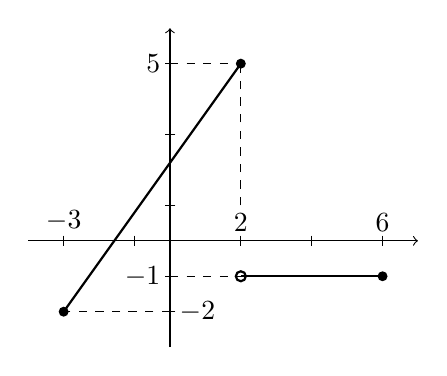
\begin{tikzpicture}[scale=0.45]
        % Eixos
        \draw[->] (-4,0) -- (7,0);
        \draw[->] (0,-3) -- (0,6);

        % Marcas
        \foreach \x in {-3,-1,2,4,6}
            \draw (\x,0.15) -- (\x,-0.15);

        \foreach \y in {-2,-1,1,3,5}
            \draw (0.15,\y) -- (-0.15,\y);

        % Rótulos principais
        \node[above] at (-3,0) {$-3$};
        \node[above] at (2,0) {$2$};
        \node[above] at (6,0) {$6$};
        \node[left] at (0,5) {$5$};
        \node[left] at (0,-1) {$-1$};
        \node[right] at (0,-2) {$-2$};

        % Segmento inclinado
        \draw[thick] (-3,-2) -- (2,5);

        % Pontos fechados
        \fill (-3,-2) circle (4pt);
        \fill (2,5) circle (4pt);

        % Segmento horizontal inferior
        \draw[thick] (2,-1) -- (6,-1);

        % Círculo aberto
        \draw[thick] (2,-1) circle (4pt);

        % Ponto fechado
        \fill (6,-1) circle (4pt);

        % Linhas auxiliares
        \draw[dashed] (2,1) -- (2,5);
        \draw[dashed] (0,-1) -- (2,-1);
        \draw[dashed] (0,-2) -- (-3,-2);
        \draw[dashed] (0,5) -- (2,5);
    \end{tikzpicture}
\end{center}

Determine o valor de \(\dfrac{f(4)+f(-3)}{f(2)-f(6)}\).

% Define as alternativas
\newcommand{\alternativas}{%
    \begin{center}
        \begin{tabularx}{\textwidth}{XXXXX}
            (a) \(-1\). &
            (b) \(-\dfrac{1}{2}\). &
            (c) \(\dfrac{1}{2}\). &
            (d) \(1\). &
            (e) \(-2\).
        \end{tabularx}
    \end{center}
}

% Define a resposta correta
\newcommand{\resposta}{B}

% Lógica condicional para exibição
\ifdefstring{\atividade}{lista}{%
    \alternativas
    \vspace{0.5em}
    
    \noindent\textbf{Resposta:} letra \textbf{\resposta}.
}{%
    \ifdefstring{\modo}{objetivo}{%
        \alternativas
    }{%
        % modo = discursiva → não mostra alternativas
    }
}
\end{exercicioBanco}

